\documentclass{article}
\usepackage[utf8]{inputenc}
\usepackage{amsmath}
\usepackage{amssymb}
\usepackage{graphicx}
\begin{document}

\section*{Complexity of a C++ function}
We consider the following \verb|C++| function
\begin{figure}[!hbt]
    \centering
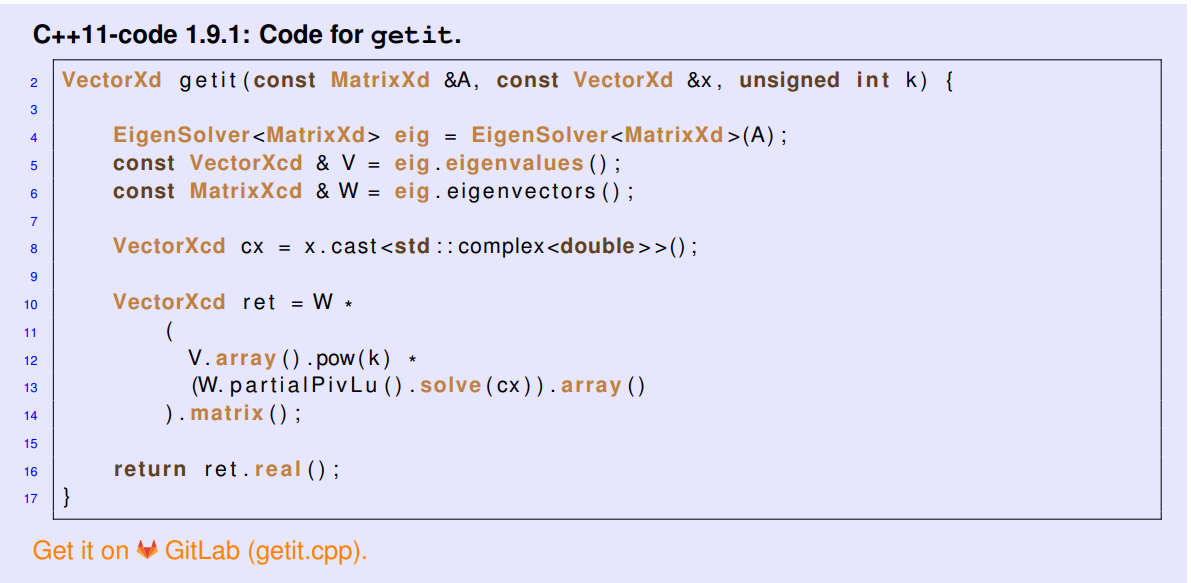
\includegraphics[width=1.0\linewidth]{1-9Code.png}
\end{figure}

\noindent Here we use \verb|EigenSolver| that computes the eigenvalues and eigenvectors of general matrices. The functions \verb|eigenvalues()| and \verb|eigenvectors()| are then used to retrieve the eigenvalues and eigenvectors respectively. We use \verb|.cast| as a built-in cast to cast between matrix types, for complex numbers we use the \verb|C++| built-in \verb|std::complex<double>|. The \verb|array()| call allows to use vectorized operations, as objects of type \verb|Eigen::ArrayXd| support them, in the example we make use of \verb|pow(k)|, others exist like \verb|sin()|, \verb|cos()|, \verb|sqrt()|, \verb|exp()|, \verb|log()|, \verb|inverse()|,  \verb|abs()|, etc. The \verb|partialPivLu()| computes the default LU-decomposition and uses partial pivoting (in contrast to \verb|fullPivLu()| which uses full pivoting. As per usual we use \verb|solve()| on the decomposition which uses forward and backward substitution to solve the system. We then multiply two array types which results in an entry wise product (as vectors this product would not be compatible). We then make a \verb|matrix()| call to transform the resulting array into a matrix again. We then return the real part of the result by using \verb|rel()| on an object of type \verb|Eigen::MatrixXcd|, which cuts of the complex part.
\subsection*{1-9.a}
We are tasked with determining what the code does if$ \mathbf{A}$ is a diagonalizable $n \times n$ matrix, $\mathbf{x \in \mathbb{R}^{n}}$ and $k \in \mathbb{N}$. Let us hence denote $\mathbf{v}$ as the vector containing the eigenvalues, $\mathbf{W}$ the matrix containing the eigenvectors, where the $i$-th entry in $\mathbf{v}$ corresponds to the $i$-th column of $\mathbf{W}$. We then cast the input vector to a complex vector which does not affect the actual values $x \in \mathbb{R}$ is now $x + 0\cdot i \in \mathbb{C}$ and hence still the same number over $\mathbb{C}$. So when doing \verb|W.partialPivLu().solve(cx)| we solve the following linear system of equations
\begin{equation*}
    \mathbf{W}\mathbf{z} = \mathbf{cx} \Longleftrightarrow \mathbf{z} = \mathbf{W}^{-1}\mathbf{cx}
\end{equation*}
This is a trick we often use, here $\mathbf{z}$ is only a placeholder that does not have any particular meaning. Let us again write this while using that $\mathbf{cx}$ and $\mathbf{x}$  are mathematically the same over the complex numbers, which then gives us 
\begin{equation*}
    \mathbf{W}\mathbf{z} = \mathbf{cx} \Longleftrightarrow 
    \mathbf{W}\mathbf{z} = \mathbf{x} \Longleftrightarrow \mathbf{z} = \mathbf{W}^{-1}\mathbf{x}
\end{equation*}
and this is the goal of this little maneuver (keep in mind that purely mathematical $\mathbf{cx}$ and $\mathbf{x}$ are the same, because every real number is also the "same" complex number) we now can proceed with $\mathbf{W}^{-1}\mathbf{x}$. We then use array operations to compute an entry-wise product, which will look as follows ($\lambda_{i}$ denote the eigenvalues and $\odot$ denotes the entry-wise product)
\begin{equation*}
\mathbf{W}\cdot\left(
\begin{bmatrix}
   \lambda_{1}^{k} \\
   \lambda_{2}^{k} \\
   \vdots \\
   \lambda_{n}^{k}
   \end{bmatrix} \odot \mathbf{W}^{-1}\mathbf{x} \right) = \left(\mathbf{W} \cdot\begin{bmatrix}
       \lambda_{1} & 0 & \dots & 0 \\
       0 & \lambda_{2} & \dots & 0 \\
       \vdots & \vdots & \ddots & \vdots \\
       0 & 0 & \dots & \lambda_{n}
   \end{bmatrix}^{k} \cdot \mathbf{W}^{-1}\right) \cdot \mathbf{x}
\end{equation*}
A entry-wise product between two vector is the same as taking a diagonal matrix with one vector on the diagonal and multiplying it with the other vector. We can see here that we do have the eigen-decomposition $\mathbf{A} = \mathbf{Q}\mathbf{\Lambda}\mathbf{Q}^{-1}$ in between the brackets given by $\mathbf{Q} = \mathbf{W}$ and 
\begin{equation*}
    \left(\mathbf{W} \cdot\underbrace{\begin{bmatrix}
       \lambda_{1} & 0 & \dots & 0 \\
       0 & \lambda_{2} & \dots & 0 \\
       \vdots & \vdots & \ddots & \vdots \\
       0 & 0 & \dots & \lambda_{n}
   \end{bmatrix}^{k}}_{= \mathbf{\Lambda}}\cdot \mathbf{W}^{-1}\right) \cdot \mathbf{x}
\end{equation*}
now we need to see that $\mathbf{A}^{k} = \mathbf{W}\mathbf{\Lambda}^{k}\mathbf{W}^{-1}$ if the eigen-decomposition exists and is given by $\mathbf{A} = \mathbf{Q}\mathbf{\Lambda}\mathbf{Q}^{-1}$. This is because the $\mathbf{W}$ matrices cancel each other out
\begin{align*}
    \mathbf{A}^{k} &= \left(\mathbf{Q}\mathbf{\Lambda}\mathbf{Q}^{-1}\right)^{k} \\
    &= \underbrace{\left(\mathbf{Q}\mathbf{\Lambda}\mathbf{Q}^{-1}\right) \cdot \left(\mathbf{Q}\mathbf{\Lambda}\mathbf{Q}^{-1}\right) \cdot \: \dots \: \cdot \left(\mathbf{Q}\mathbf{\Lambda}\mathbf{Q}^{-1}\right)}_{k\text{- times}} \\
    &= \mathbf{Q}\mathbf{\Lambda}\big(\underbrace{\mathbf{Q}\mathbf{Q}^{-1}}_{= \mathbf{I}}\big)\mathbf{\Lambda}\big(\underbrace{\mathbf{Q}\mathbf{Q}^{-1}}\big) \dots \mathbf{\Lambda}\big(\underbrace{\mathbf{Q}\mathbf{Q}^{-1}}\big)\mathbf{\Lambda}\mathbf{Q}^{-1} \\
    &= \mathbf{Q}\mathbf{\Lambda}^{k}\mathbf{Q}^{-1}
\end{align*}
and hence we compute $\mathbf{A}^{k}\mathbf{x}$. This is one of the most efficient ways to compute powers of matrices (ignoring multiplying with $\mathbf{x}$), this can however only be done if the eigen-decomposition exists.
\subsection*{1-9.b}
We are tasked with stating the asymptotic complexity of the given code. We get the decomposition from \verb|EigenSolver| in $\mathcal{O}\left(n^{3}\right)$ as we are told by the exercise description, retrieving the vectors amounts to $\mathcal{O}\left(n\right)$ cost as we must set their entries, casting the vector will amount at most to $\mathcal{O}\left(n\right)$ computational cost. We then compute the powers of $\mathbf{v}$ entry wise which gives $\mathcal{O}\left(n\right)$ cost, getting the LU decomposition takes $\mathcal{O}\left(n^{3}\right)$ and solving the system takes $\mathcal{O}\left(n^{2}\right)$, the array multiplication takes $\mathcal{O}\left(n\right)$ because it is entry-wise multiplication. The final product between $\mathbf{W}$ and the big term takes $\mathcal{O}\left(n^{2}\right)$ because it is a matrix-vector product. Returning the real part of the result vector will take at most $\mathcal{O}\left(n\right)$ time and hence overall we get an asymptotic complexity of $\mathcal{O}\left(n^{3}\right)$.
\end{document}
